% !TeX root = thesis.tex
\documentclass{master_thesis}
\addbibresource{refs.bib}

\begin{document}

\section{Theoretical Background}\label{chap:background}

This chapter aims to provide a comprehensive summary of the concepts and principles that are relevant to this research. This includes giving an overview of accessibility, including the tools and methodologies used to evaluate it, the format for defining testable accessibility rules, and the concept of component libraries, their purpose and their importance in contemporary software engineering practices.

\subsection{Web Accessibility}

Accessibility is about providing equal access to goods and services to everyone regardless of age, gender, knowledge or disabilities. We all have different abilities, some run faster than others, some see more clearly and some might not be able to hear sounds. A report published by the European Commission in \citeyear{Grammenos2020} estimates that approximately 7\% of people aged 16 and over living in the EU have a severe disability, and about 17.5\% have a moderate disability \citep{Grammenos2020}. This number gets significantly higher as people get older. Disability prevalence among people aged 65 and over is about 47.8\%.  Disability is a part of being human and people with disabilities have very different needs. In addition, temporary disabilities should also be considered - these might include a mother who can only use one hand because she is holding a child in the other or someone who broke an arm and can't use it until it heals. The experiences during a temporary disability may be very similar to a permanent condition. Everyone who designs the physical and virtual environment around us should consider these different limitations.

Accessibility principles can be applied to various fields. For example, in architecture, it could be designing buildings in a way that can be accessed by people who can walk as well as the ones who need to use a wheelchair. In digital products, it is more often related to the senses we use to navigate and consume content. Everything should be equally accessible regardless of the sense someone wants or needs to use for consuming the information.

The biggest strength of the web lies in its availability to everyone. Tim Berners-Lee, \ac{wcag} Director and inventor of the World Wide Web has said: "The power of the Web is in its universality. Access by everyone regardless of disability is an essential aspect" \citep{WWWC1997}. The virtual world has the potential to be much more inclusive than the physical world.

Web accessibility considers auditory, cognitive, neurological, physical, speech and visual disabilities - everything that might affect someone's ability to access the web and people using different devices, who have reduced abilities because of aging, temporary disabilities, situational limitations or are using limited or slow internet or devices \citep{Henry2022}.

\subsubsection{Web Accessibility Standards}

The most commonly used standard for considering people with different abilities and making web content accessible for different ways of consuming is defined in \ac{wcag} \citep{Kirkpatrick2018}. The guidelines are developed by \ac{wai} which is part of \ac{w3c}.

The first version of \ac{wcag} (1.0) was published in 1998 \citep{Vanderheiden1998}. The current version is \ac{wcag} 2.1 and the next version 2.2 is scheduled to be finalized in May 2023 \citep{Henry2023}. All \ac{wcag} versions are backward compatible, meaning that all requirements that were in 2.0 are included in 2.1 and some new requirements are added. Version 2.2 is currently in the draft stage, but the planned changes also include some minor changes to the current guidelines. This means version 2.2 will not be entirely backward compatible with the previous versions.

Discrimination against disabled people is addressed in various laws and directives around the world. Many of them are based on or derived from some version of \ac{wcag}. Pipedrive operates in the United States and Europe, making these regulations most relevant to this case study.

In the United States accessibility is addressed in two laws \citep{Siteimprove}. Amendment of Section 508 includes \ac{wcag} and regulates accessibility related to Federal agencies and organizations that receive federal funds or are employed under contract with a federal agency. Title III of the Americans with Disabilities Act ensures that public goods and services are equally accessible to everyone.

European Union has two directives that outline what accessibility should look like and leave it to each member state to make national laws based on that. European Union Web Accessibility Directive states that the public sector should follow EN 301 549 which includes \ac{wcag} 2.1 Level AA and European Accessibility Act aims to ensure that essential products and services traded in and between European Union member states are equally accessible to everyone.

\ac{wai} gives an overview of the laws and policies around the world. 25 out of 40 laws and policies listed on their webpage are based on \ac{wcag} 2.0 or \ac{wcag} 2.0 derivative \citep{Mueller2018}. This thesis will use \ac{wcag} 2.1 as the basis for all evaluations, given that it is the latest published version of the most commonly used accessibility standard.

\ac{wcag} is intended for anyone who is involved in developing web content, authoring tools or web accessibility evaluation tools and others who need a standard for accessibility \citep{Henry2023}. The 4 principles of accessibility addressed in the guidelines are:
\begin{enumerate}
	\item Perceivable - information and user interface should be presented in a way that users don't have to rely on a single sense to perceive it.
	\item Operable - user should be able to interact with the interface.
	\item Understandable - user should understand the information and how the user interface operates.
	\item Robust - content should be robust enough that it can be interpreted reliably by a wide variety of user agents and assistive technology.
\end{enumerate}
Under each principle is a list of guidelines that address that principle \citep{AGWGWP2022}. Under each guideline, there are Success Criteria that describe specifically what conformance to it means. Each Success Criterion is a statement that will be either true or false for a specific web content.

\subsubsection{Web Accessibility Rules Format}

\ac{w3c} Accessibility Guidelines Working Group has developed \ac{act} Rules Format to provide developers of evaluation methodologies and testing tools a consistent interpretation of how to test for conformance with accessibility requirements like \ac{wcag} \citep{Fiers2019}. The format describes both manual and automated tests. The aim of this is to make accessibility tests transparent and results reproducible.

For example, accessibility testing tools check if the provided \ac{html} meets the requirements defined in \ac{wcag}. These requirements are different for each element, but they might be also combined and include more criteria. Each element needs a specific set of requirements to be checked.

\ac{act} Rules include atomic rules that define an element to be tested for a single condition and composite rules that can combine multiple atomic rules to determine if a single test subject satisfies an accessibility requirement \citep{Fiers2019}. Each rule defines when it should be applied. In the case of an atomic rule, this might be an \ac{html} tag name, computed role, or distance between two elements. For composite rules, applicability is determined by a union of the atomic elements that it combines.

\subsection{Accessibility Evaluation}

Different evaluation methods are used to determine if a website, digital document or mobile application is accessible. These include expert review, user testing, subjective assessment, screening techniques or barrier walkthrough. Each method has its pros and cons depending on the subject of the evaluation, available experts and other factors.

Expert review - also called conformance, standards or guidelines review, or manual inspection - is the most widely used method \citep{Brajnik2008}. It involves analyzing web content to verify whether it meets a list of criteria. The results depend on the evaluator's opinions and the chosen guidelines. Skillful evaluators are needed for this method to be effective.

Barrier walkthrough is a technique where the evaluator has to assess how seriously some predefined barriers impact the user in achieving their goal on the website \citep{Brajnik2008}. An accessibility barrier can be any condition that makes it difficult for a person to achieve a goal.

Screening techniques consist of evaluating a website by using the interface while some sensory, motor or cognitive capabilities of the user are artificially reduced \citep{Brajnik2008}. Subjective assessment is based on a panel of users exploring a website by themselves and giving feedback on what worked and what did not. User testing means conducting usability tests with disabled people while adopting a think-aloud method to get feedback on their experience.

Which method is suitable depends on several factors, including the availability of skilled auditors and other resources. Evaluations with experts are very dependent on the knowledge and experience of the evaluators. Research into the effect of expertise on web accessibility evaluation conducted by \citeauthor{Brajnik2011} shows that when web pages are evaluated with non-experts we see a drop in reliability and validity \citep{Brajnik2011}. Even with experts, the result will vary, but the results should even out when at least 3 experts are used. For the same level of reliability, at least 14 evaluators that are not considered experts in the field of web accessibility are needed.

Manual testing with experts or users is essential to making websites truly accessible to everyone. Currently, there is no tool available that can replace human evaluation of many \ac{wcag} success criteria. For example, determining if the link text is informative enough or if an input field's error message suggests what needs to be corrected clearly enough.

\subsubsection{Tools for Accessibility Evaluation}

There are software programs and online services that help determine if web content meets accessibility guidelines. These tools may be browser or authoring tool plugins, command line tools, code linters, open source \ac{api}, desktop or mobile applications or online services \citep{AbouZahra2017}. Some tools are aimed at non-technical content creators and are often built into the tools they use daily. Others are online services, where the user can enter the URL of the website to be evaluated or services that regularly check the website and are hosted by the provider or in a company's internal network. These tools may support various accessibility standards.

The results can be presented as a report in HTML, CVS, PDF, XML or other formats, as in-page feedback with temporary icons and markup or as a step-by-step evaluation where the user is prompted to assess the parts that can't be automated \citep{AbouZahra2017}. The tool might transform the page, show only text or take away all the colors, for example, to help identify issues. These tools can usually evaluate either a single page or a group of related pages at the same time. Some tools are even capable of accessing password-protected content.

Browser extensions and online tools usually evaluate one page at a time. This might work well for small websites and one-time audits but can be quite ineffective to use as a continuous solution. \Ac{cli} tools need more setup, but can potentially be seamlessly integrated into the development workflow.

\begin{figure}[ht]
	\centering
	\begin{subfigure}{0.4\textwidth}
		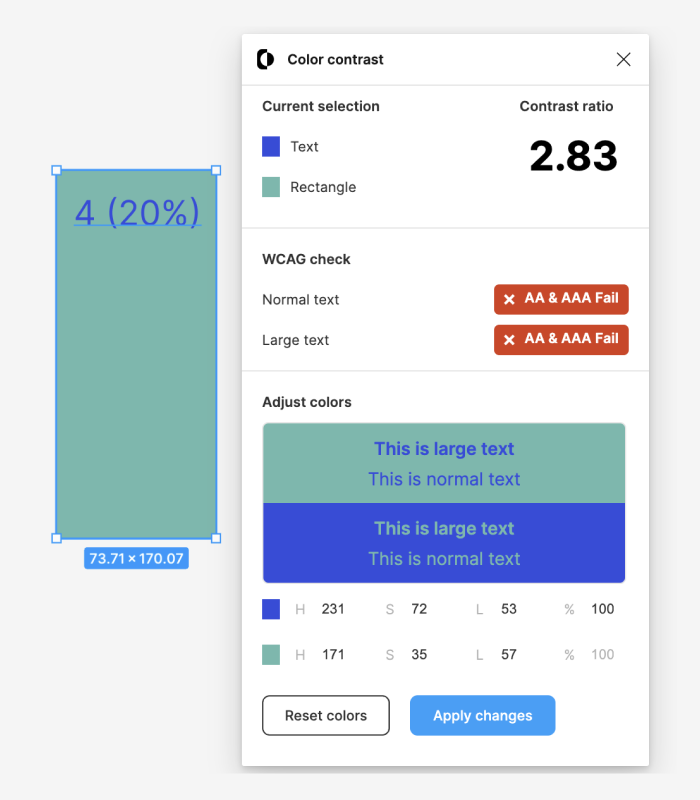
\includegraphics[width=\textwidth]{img/figma plugin-color-contrast-fail.png}
		\caption{Color contrast test failing}
	\end{subfigure}
	\hspace{0.05\textwidth}
	\begin{subfigure}{0.4\textwidth}
		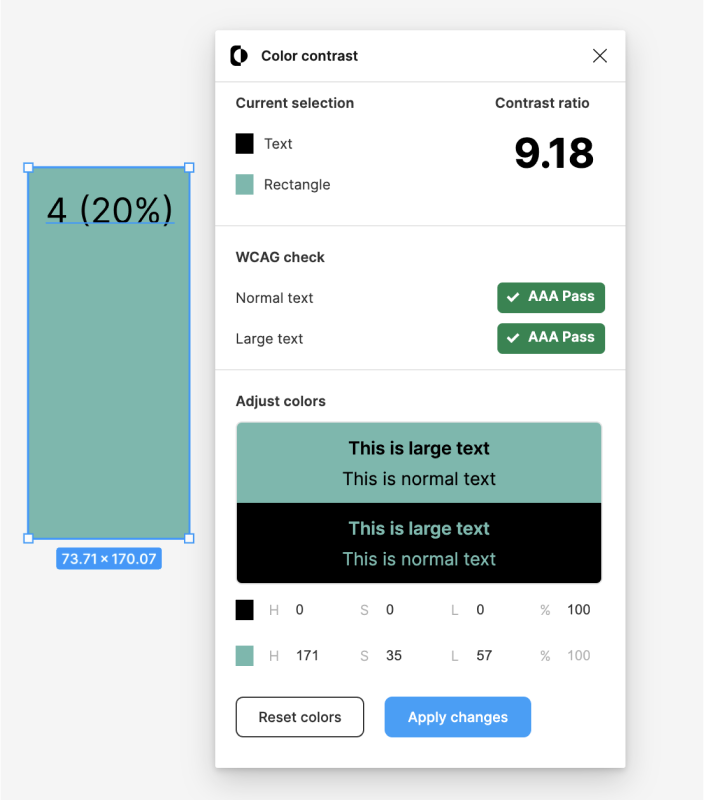
\includegraphics[width=\textwidth]{img/figma plugin-color-contrast-pass.png}
		\caption{Color contrast test passing}
	\end{subfigure}
\caption{Figma plugin for testing color contrast compliance with \ac{wcag}}
\label{fig:figma-plugin}
\end{figure}

Authoring tool plugins can be, for example, plugins for Figma that check if the colors used in the design conform with \ac{wcag} requirements (Figure \ref{fig:figma-plugin}) or plugins for integrated development environments that provide immediate feedback to developers when they miss something related to accessibility in their code.

Some tools do a very specific task or work inside a very certain tool and others try to tackle accessibility as thoroughly as possible. In most cases, using many different tools in combination will give the best result.

\subsubsection{Continuous Accessibility Evaluation} \label{continuous-a11y-evaluation}

\Ac{ci} is a software development practice where members of the team integrate their work frequently and each integration is verified with an automated build that includes tests to detect errors as quickly as possible. This is believed to help develop high-quality software more rapidly \citep{Fowler2006}. One of the practices in \ac{ci} is making your code self-testing - adding a suite of automated tests that can check a large part of the codebase for bugs. These tests need to be easy to trigger and indicate any failures.

This last principle could be applied well to accessibility evaluation while following modern software development principles. The automated tests will not catch all accessibility issues, but they will catch enough to make it worthwhile. After the initial setup, they should not need a lot of maintenance and would be run every time someone contributes to the codebase. This can act as a very effective gatekeeper for any potential accessibility issues.

Tools that can be set up to perform checks automatically with minimal manual effort every time changes are made to the code, can be used for continuous accessibility testing. The earlier these can be triggered in the development process, the better. Not all of the tools described in the previous chapter can be used for that, for example, browser extensions and plugins in authoring tools need to be manually triggered to perform checks. \ac{cli} based tools are the most suitable for continuous accessibility testing.

\ac{cli} tools can be customized to meet specific needs and integrated to run together with other tests. The \ac{dom} is the data representation of the objects that comprise the structure and content of a document on the web \citep{MDN2023}. CLI tools scan the rendered \ac{dom} of a website against accessibility standards like \ac{wcag} to find violations. The errors are reported back with a reference to the code that produced the error and, in most tools, a link to the accessibility rule it violated.

According to the survey conducted by one of the leading digital accessibility solution providers - Level Access about the state of digital accessibility, 67\% of organizations that practice \ac{ci} also include accessibility tests \citep{LevelAccess}. This has gone up from 56\% reported in 2021. 91\% of all organizations that participated in the survey say they use accessibility testing tools and most of them prefer the free options available. The survey states that browser extensions are by far the most popular tool with 82.4\% of organizations using them. 23.4\% of organizations reported that they use testing technology that integrates with their \ac{ci} tool and 22.7\% uses testing technology that is compatible with their test framework. Level Access's survey results show that organizations that have an accessibility program in its early stages (2-6 years) or have \ac{iaap}-certified personnel are more likely than the average to have implemented a \ac{ci} accessibility testing process.

It is important to mention that automated tests can detect only a part of all the possible violations. The UK Government Digital Service Accessibility team compared 13 automated tools' performance in \citeyear{GAT2018} on a page that had 142 deliberately introduced accessibility issues and found that the different automated tools were able to detect 13-40\% of issues. \citeauthor{Abbott2021} compared the two most popular accessibility tools that can be used in \ac{ci} using the same deliberately inaccessible site in \citeyear{Abbott2021} and reported that axe-core caught 27\% and pa11y 20\% \citep{Abbott2021}. \citeauthor{Vigo2013} compared 6 different tools in \citeyear{Vigo2013} and found that they were able to detect 23-50\% of  \ac{wcag} 2.0 Success Criteria \citep{GAT2018, Abbott2021, Vigo2013}.

The tools and \ac{wcag} standards have evolved during this time, but the common conclusion to most of the similar comparisons is still that, most tools will be able to detect errors on 20-30\% or \ac{wcag} Success Criteria.

Axe-core accessibility testing engine promises to find on average 57\% issues, which is significantly higher than other tools on the market. To understand this Deque Systems took a look at how coverage is defined and measured. They claim that the current statistics are founded on an inaccurate definition of accessibility coverage - the percentage of individual \ac{wcag} Success Criteria \citep{Deque2023}. According to Deque Systems, in reality, some types of issues are found much more frequently and the issues found by automated tests form a higher percentage of all issues compared to those discovered by manual detection. They suggest that the coverage should be the percentage of all the issues found on a site. To prove the validity of this way of calculating the coverage of accessibility tests, a study was conducted where 2000 axe-core and manual testing audit results were compared \citep{DequeSystems2021report}. The results show that the average percentage of issues detected by axe-core is 57.38\%.

In the report, they also state that with the current, in their opinion, inaccurate definition of the coverage, the results would be in the range of 20-30\% \citep{DequeSystems2021report}. No studies about other tools that would have used the same method for calculating the coverage were found so in this paper percentage of tested WCAG Success Criteria will be used when making comparisons between different accessibility evaluation tools.

There is still a limit to what can be detected no matter how we define the coverage. There are aspects of accessibility that need human interpretation. The tools that are currently available can't interpret how well image alternative conveys the meaning of the image or even if the image on the webpage is purely decorative or a part of meaningful content. The goal of using automated testing tools should be to help make the testing process easier by catching problems that can be detected automatically. This gives the human evaluator more time to focus on the remaining issues.

Manual testing will always be required to ensure that the content is fully accessible. The main strengths of automated tests are that they can be set up to run automatically and provide measurable results. Therefore, it is a good way to monitor compliance with \ac{wcag} rules consistently without much extra effort. This can help avoid unwanted changes and highlight issues in code that should be straightforward to fix.

\subsection{Component Libraries}

% \todo{ start from design systems \citep{Churchill2019}}

\ac{cdd} is a development methodology that anchors the build process around components \citep{Coleman2017}. In \citeyear{Coleman2017} \citeauthor{Coleman2017} called \ac{cdd} the biggest trend in \ac{ui} development.

A component is a well-defined and independent piece of \ac{ui}, like a button, checkbox or card \citep{Ella2019}. This approach correlates well with other similar widespread principles that promote modularity in software development like atomic design and micro-front-ends. Designing each component as a standalone unit improves maintenance, reusability, and testing, shortens the learning curve and makes development faster. The key to success here is the separation of concerns and isolating a logical piece so that it can be worked on without distractions. \ac{cdd} promotes concentrating on details and refining the element as much as possible. These pieces can be combined into more complex components if needed, and when combined, they can make up views that become the whole site or web page.

It is not very straightforward to preview one single component on its own and if you needed to set up a test or live environment for the whole webpage it would defeat the purpose of dividing the big problem into manageable chunks. In development, tools called component explorers are often used to mitigate that.

Component Explorer is a separate application that showcases the components in various states \citep{Coleman2017}. Without a tool like that developers would often need to manipulate the entire webpage or app to a certain state just to work on a single component. A Component Explorer allows developers to test a given component in isolation and make it easy to build one component at a time. It also makes it easier to go through all the possible states in one component and promotes the reusability of these elements.

Bit, Storybook and Styleguidist are popular tools used in component library development \citep{Ella2019}. Bit allows the user to pack the bundled and encapsulated components and share them on the cloud where the team can visually explore them. Storybook supports multiple frameworks and provides a rapid component development and test environment. The environment also allows you to present and document your library for better reusability. Styleguidist is useful for documentation and demoing different components.

Design Systems are a popular way to help companies scale design work and build products with consistent user experience \citep{Yew2020}. \citeauthor{Yew2020} defines it as: "...a repository of reusable components that follow a set of shared design principles". Many companies build their own design systems. A design system should include a component library, style guide, design and content guidelines, design token library, interactive prototyping tools and accessibility guidelines.

Many big companies have a design system with an open source code that includes a component library, making it possible to reuse and extend the components. Some of the more known ones include Material-UI \citep{MUS}, Adobe Spectrum \citep{Adobe} and Bootstrap \citep{Collings}.

% These all work together to help keep things consistent across multiple projects by providing small building blocks that can be used to create complex designs.  It can be built with \ac{html} or by using a framework like React or Vue.

% Component libraries are a part of the company's Design System.  Design systems include values and principles along, with branding, guidelines and all the building blocks and design patterns to create a successful product or service. It governs the design process in the organization. A component library or \ac{ui} kit, \ac{ui} library, and \ac{ui} component library are one of the building blocks of a design system.


Using a component library provides consistency and better design and code quality. These components can be polished over time to provide the best user experience when they are integrated into the final product. The effort that can be put into developing a component that will be used in multiple projects is bigger than what would be reasonable for a single use case.

\end{document}
